%!TEX root = ../thesis.tex

\section{背景}
近年, 機械学習を用いた自律走行に関する研究が盛んにされており, その中でカメラ画像を用いてロボットへ自律走行を行わせる研究もされている. Bojarskiら\cite{bojarski}は\figref{Fig:bojarski_train}に示すシステムで, 人間のドライバーが操作するステアリング角度と前方カメラ画像を用いて模倣学習を行った. また, \figref{Fig:bojarski_test}に示すように, 訓練したネットワークに画像を入力し, 生成される操舵指令を用いて走行を行う手法を提案した.

\vspace{0.5cm}

\begin{figure}[hbtp]
  \centering
 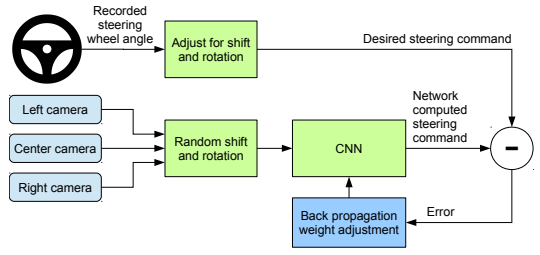
\includegraphics[keepaspectratio, scale=0.9]
      {images/bojarski_train.png}
 \caption{Training the neural network from \cite{bojarski}}
 \label{Fig:bojarski_train}
\end{figure}

\begin{figure}[hbtp]
     \centering
    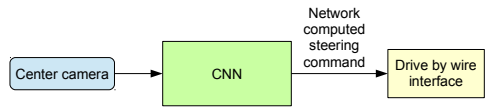
\includegraphics[keepaspectratio, scale=0.7]
         {images/bojarski_test.png}
    \caption{The trained network is used generate steering commands from a single front-facing center camera from \cite{bojarski}}
    \label{Fig:bojarski_test}
\end{figure}

\newpage

本研究室においても, 岡田ら\cite{okada1}は\figref{Fig:okada_structure}に示すようなシステムを用いて\figref{Fig:okada_nav}のように経路追従行動を模倣学習し, カメラ画像に基づいた経路追従行動を獲得した. このシステムでは, LiDAR, オドメトリを入力としたルールベース制御器(後述する”地図を用いたルールベース制御器”)による経路追従行動を前方カメラ画像を用いてend-to-endで模倣学習した. 

\vspace{2.5cm}

\begin{figure}[hbtp]
     \centering
     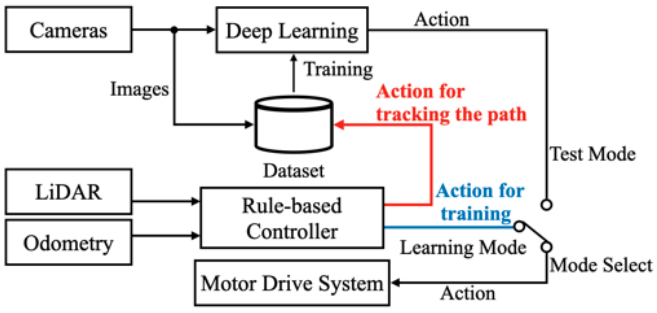
\includegraphics[keepaspectratio, scale=0.55]
          {images/okada_structure.png}
     \caption{Structure of the proposed system from \cite{okada1}}
     \label{Fig:okada_structure}
\end{figure}

\begin{figure}[hbtp]
     \centering
    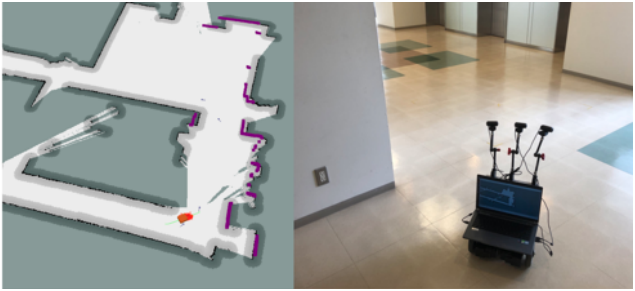
\includegraphics[keepaspectratio, scale=0.5]
         {images/okada_nav.png}
    \caption{A robot that follows a path using vision based on the proposed method from \cite{okada1}}
    \label{Fig:okada_nav}
\end{figure}

\newpage

上記の研究により, カメラ画像に基づいてロボットが学習した経路を周回可能であることが確認されている. 次に岡田ら\cite{okada1}の研究(以下, 「従来手法」と称する)をベースに, \figref{Fig:road}のような進む方向が一意ではない分岐路において, 任意の経路を選択する機能の追加を検討する.

\vspace{1cm}

\begin{figure}[hbtp]
     \centering
    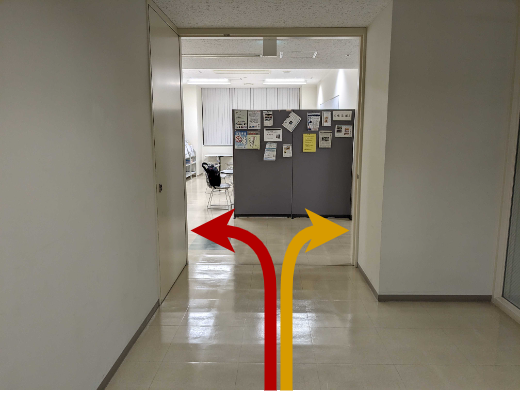
\includegraphics[keepaspectratio, scale=0.5]
         {images/road.png}
    \caption{A fork in the road where the direction of travel is not unique}
    \label{Fig:road}
\end{figure}

\newpage

本研究では, 従来手法をベースに「直進」, 「左折」, 「右折」の目標とする進行方向の情報(以下, 「目標方向」と称する)をデータセットと学習器へ与える. これにより, 訓練済みの学習器の出力を用いた走行において, 目標方向により任意の経路を選択可能とする機能の追加を提案する. 提案手法全体の流れをfigに示す.

\newpage
